
As a starting example, we consider a compartment pharmacokinetic model for a single patient.
The patient receives multiple doses at regular time intervals and the drug plasma concentration is recorded over time.
Our goal is to infer the physiological parameters of the patient, pertinent to the drug's pharmacokinetics, and the measurement error.

\subsection{Pharmacokinetic model and clinical event schedule} \label{sec:twocpt}

The two compartment pharmacokinetic model describes how the drug circulates in the patient's body, until it is cleared out (Figure~\ref{fig:twocpt}).
The drug is orally administered and enters the system through the gut.
Once the drug is introduced in the system, the \textit{natural evolution} of the system is described by a system of ODEs.
In the case of a two compartment model with a first-order absorption from the gut, the system is the following:
%
\begin{subequations}
\begin{eqnarray*}
  \frac{\mathrm d y_\mathrm{gut}}{\mathrm d t} & = & - k_a y_\mathrm{gut} \\ 
  \frac{\mathrm d y_\mathrm{cent}}{\mathrm d t} & = & k_a y_\mathrm{gut} - \left (\frac{CL}{V_\mathrm{cent}} + \frac{Q}{V_\mathrm{cent}} \right) y_\mathrm{cent} + \frac{Q}{V_\mathrm{peri}} y_\mathrm{peri} \\
  \frac{\mathrm d y_\mathrm{peri}}{\mathrm d t} & = & \frac{Q}{V_\mathrm{cent}} y_\mathrm{cent} - \frac{Q}{V_\mathrm{peri}} y_\mathrm{peri}
\end{eqnarray*}
\label{eq:twocpt}
\end{subequations}
%
with
\begin{itemize}
  \setlength\itemsep{0em}
  \item $y(t)$: the drug mass in each compartment (mg),
  \item $k_a$: the rate constant at which the drug flows from the gut to the central compartment (h$^{-1}$),
  \item $Q$: the clearance at which the drug flows back and forth between the central and the peripheral compartment (L/h),
  \item $CL$: the clearance at which the drug is cleared from the central compartment (L / h),
  \item $V_\mathrm{cent}$: the volume of the central compartment (L),
  \item $V_\mathrm{peri}$: the volume of the peripheral compartment (L).
\end{itemize}

\begin{figure}
  \begin{center}
  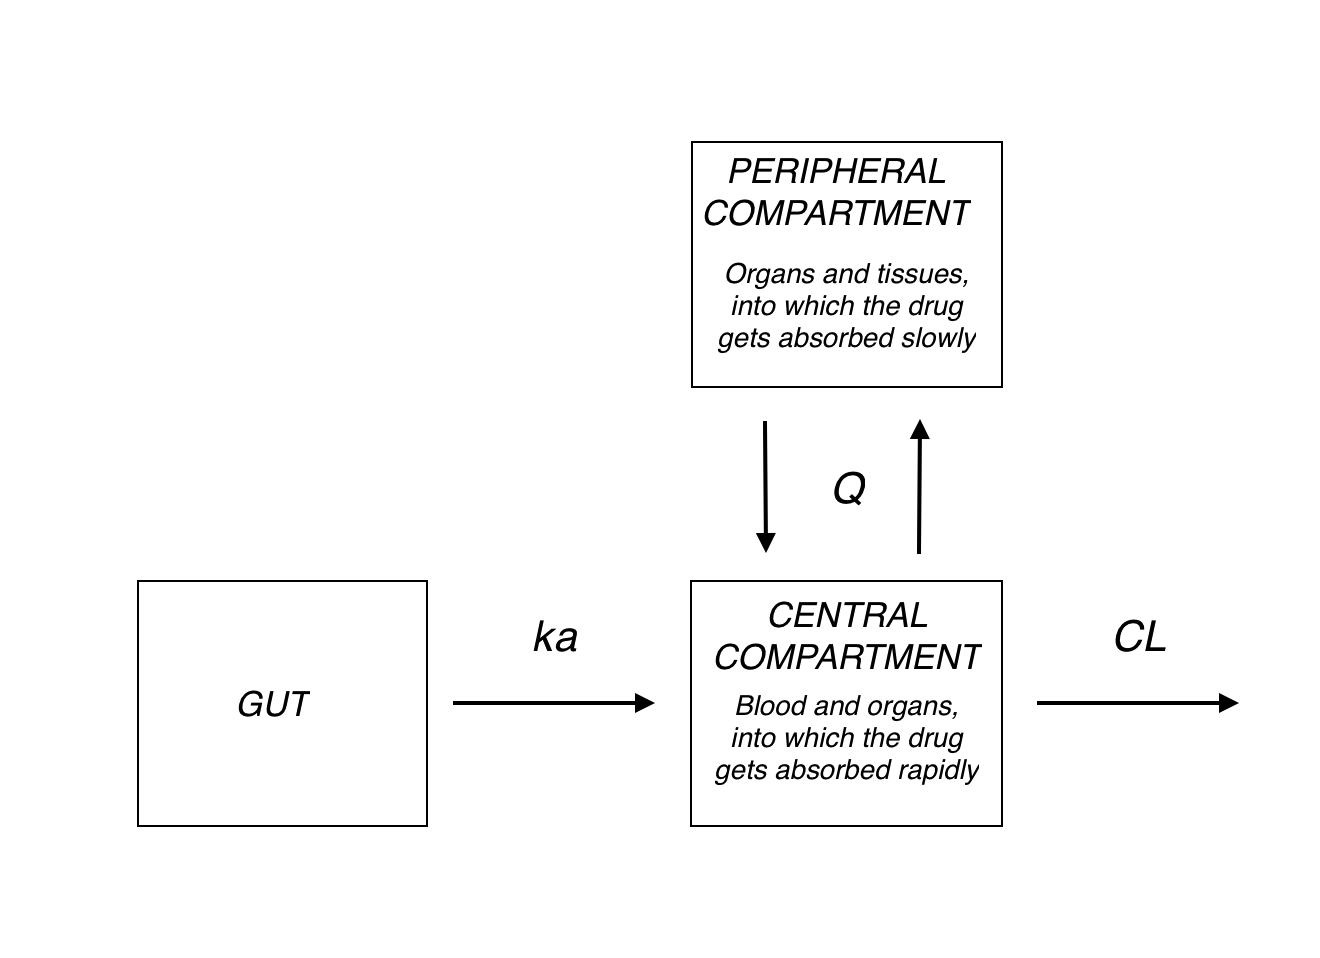
\includegraphics[width=5in]{../figures/TwoCptNice.png}
  \caption{Two compartment model with first-order absorption from the gut.}
  \label{fig:twocpt}
  \end{center}
\end{figure}

During the trial, the patient receives a dose of 1,200 mg every 12 hours, until they have received a total of 14 doses.
Measurements are taken shortly after the first, second, and last doses, and at regular intervals during the treatment.
Both intervention and measurement events are described by the event schedule, which follows the convention established by NONMEM.
This means the user must provide for each event the following variables: \texttt{cmt}, \texttt{evid}, \texttt{addl}, \texttt{ss}, \texttt{amt}, \texttt{time}, \texttt{rate}, and \texttt{ii}.
Table~\ref{tab:event_schedule} provides an overview of the roll of each variable and more details can be found in the \textit{Torsten User Manual}.

\begin{table}
  \renewcommand{\arraystretch}{1.5}
  \begin{center}
  \begin{tabular} {l l l}
  \rowcolor[gray]{0.95} \textbf{Variable} & \textbf{Description} \\
  \texttt{cmt} & Compartment in which event occurs.\\
  \rowcolor[gray]{0.95} \texttt{evid} & Type of event: (0) measurement, (1) dosing. \\
  \texttt{addl} & For dosing events, number of additional doses.  \\
  \rowcolor[gray]{0.95} \texttt{ss} & Steady state indicator: (0) no, (1) yes. \\
  \texttt{amt} & Amount of drug administered. \\
  \rowcolor[gray]{0.95} \texttt{time} & Time of the event. \\
  \texttt{rate} & For dosing by infusion, rate of infusion. \\
  \rowcolor[gray]{0.95} \texttt{ii} & For events with multiple dosing, inter-dose interval.
  \end{tabular}
  \end{center}
  \caption{Available variables in Torsten to specify an event schedule.}
  \label{tab:event_schedule}
\end{table}

\subsection{Statistical model}

% We define a generative model.
Given a treatment, $x$, and the physiological parameters, $\{ k_a, Q, CL, V_\mathrm{cent}, V_\mathrm{peri} \}$, we compute the drug plasma concentration, $\hat c$, by solving the relevant ODEs.
Our measurements, $y$, are a perturbation of $\hat c$.
This is to account for the fact that our model is not perfect and that our measurements have finite precision.
We model this residual error using a lognormal distribution, that is
\begin{equation*}
  y \mid \hat c, \sigma \sim \mathrm{logNormal}(\log \hat c, \sigma^2),
\end{equation*}
where $\sigma$ is a scale parameter we wish to estimate.
The deterministic computation of $\hat c$ along with the measurement model, defines our likelihood function $p(y \mid \theta, x)$, where $\theta = \{ k_a, Q, CL, V_\mathrm{cent}, V_\mathrm{peri}, \sigma \}$.

It remains to define a prior distribution, $p(\theta)$.
Our prior should allocate probability mass to every plausible parameter value and exclude patently absurd values.
For example the volume of the central compartment is on the order of ten liters, but it cannot be the size of the Sun.
In this simulated example, our priors for the individual parameters are based on population estimates from previous (hypothetical) studies.
\begin{eqnarray*}
  CL & \sim & \mathrm{logNormal}(\log(10), 0.25);  \\
  Q & \sim & \mathrm{logNormal}(\log(15), 0.5); \\
  V_\mathrm{cent} & \sim & \mathrm{logNormal}(\log(35), 0.25); \\
  V_\mathrm{peri} & \sim & \mathrm{logNormal}(\log(105), 0.5); \\
  k_a & \sim & \mathrm{logNormal}(\log(2.5), 1); \\
  \sigma & \sim & \mathrm{Half-Normal}(0, 1); \\
\end{eqnarray*}

Suggestions for building priors can be found in references \cite{Gabry:2019, Betancourt:2020} and at \url{https://github.com/stan-dev/stan/wiki/Prior-Choice-Recommendations}.

\subsection{Specifying a model in Stan}

We can now specify our statistical model using a Stan file, which is divided into coding blocks, each with a specific role.
From R, we then run inference algorithms which take this Stan file as an input.

\subsubsection{Data and parameters block}

To define a model, we need a procedure which returns the log joint distribution, $\log p(\mathcal D, \theta)$.
Our first task is to declare the data, $\mathcal D$, and the parameters, $\theta$, using the coding blocks \texttt{data} and \texttt{parameters}.
It is important to distinguish the two.
The data is fixed.
By contrast, the parameter values change as HMC explores the parameter space, and gradients of the joint density are computed with respect to $\theta$, but not $\mathcal D$.

For each variable we introduce, we must declare a type and, for containers such as arrays, vectors, and matrices, the size of the container.
In addition, each statement ends with a semi-colon.
It is possible to specify constraints on the parameters, using the keywords \texttt{lower} and \texttt{upper}.
If one of these constraints is violated, Stan returns an error message.
More importantly, constrained parameters are transformed into unconstrained parameters -- for instance, positive variables are put on the log scale -- which greatly improves computation.

\begin{lstlisting}[style=stan, numbers=none] 
  data {
    int<lower = 1> nEvent;
    int<lower = 1> nObs;
    int<lower = 1> iObs[nObs];  // index of events which
                                // are observations.

    // Event schedule
    int<lower = 1> cmt[nEvent];
    int evid[nEvent];
    int addl[nEvent];
    int ss[nEvent];
    real amt[nEvent];
    real time[nEvent];
    real rate[nEvent];
    real ii[nEvent];

    // observed drug concentration
    vector<lower = 0>[nObs] cObs;
  }
  
  parameters {
    real<lower = 0> CL;
    real<lower = 0> Q;
    real<lower = 0> VC;
    real<lower = 0> VP;
    real<lower = 0> ka;
    real<lower = 0> sigma;
  }
\end{lstlisting}

\subsubsection{model block}

Next, the \texttt{model} block allows us to modify the variable \texttt{target}, which Stan recognizes as the log joint distribution.
The following statement increments \texttt{target} using the prior on $\sigma$, which is a normal density, truncated at 0 to only put mass on positive values.
\begin{lstlisting}
target += normal_lpdf(sigma | 0, 1);
\end{lstlisting}
The truncation is implied by the fact $\sigma$ is declared as lower-bounded by 0 in the parameters block.
An alternative syntax is the following:
\begin{lstlisting}
sigma ~ normal(0, 1);
\end{lstlisting}
This statement now looks like our statistical formulation and makes the code more readable.
But we should be mindful that this is not a sampling statement, rather instructions on how to increment \texttt{target}.
We now give the full model block:
\begin{lstlisting}
model {
  // priors
  CL ~ lognormal(log(10), 0.25); 
  Q ~ lognormal(log(15), 0.5);
  VC ~ lognormal(log(35), 0.25);
  VP ~ lognormal(log(105), 0.5);
  ka ~ lognormal(log(2.5), 1);
  sigma ~ normal(0, 1);

  // likelihood
  cObs ~ lognormal(log(concentrationHat[iObs]), sigma);
}
\end{lstlisting}
%
The likelihood statement involves a crucial term we have not defined yet: \texttt{concentrationHat}.
Additional variables can be created using the transformed data and transformed parameters blocks.
We will take advantage of these to compute the drug concentration in the central compartment for each event.
Note that for the likelihood, we only use the concentration during observation events, hence the indexing \texttt{[iObs]}.

\subsubsection{Transformed data and transformed parameters block} \label{sec:twocpt_transformed_parameters}

In \texttt{transformed data}, we can construct variables which only depend on the data.
For this model, we simply specify the number of compartments in our model (including the gut), \texttt{nCmt}, and the numbers of physiological parameters, \texttt{nTheta}, two variables which will come in handy shortly.
\begin{lstlisting}
  transformed data {
    int nCmt = 3;
    int nTheta = 5; 
  }
\end{lstlisting}
%
Because the data is fixed, this operation is only computed once.
By contrast, operations in the \texttt{transformed parameters} block need to be performed (and differentiated) for each new parameter values.

To compute \texttt{concentrationHat} we need to solve the relevant ODE within the clinical event schedule.
Torsten provides a function which returns the drug mass in each compartment at each time point of the event schedule.
\begin{lstlisting}
matrix<lower = 0>[nCmt, nEvent] 
  mass = pmx_solve_twocpt(time, amt, rate, ii, evid,
                          cmt, addl, ss, theta);
\end{lstlisting}
%
The first eight arguments define the event schedule and the last argument, \texttt{theta}, is an array containing the physiological parameters, and defined as follows:
\begin{lstlisting}
real theta[nTheta] = {CL, Q, VC, VP, ka};
\end{lstlisting}
%
It is also possible to have \texttt{theta} change between events, and specify lag times and bio-availibilities fractions, although we will not take advantage of these features in the example at hand.

The Torsten function we have chosen to use solves the ODEs analytically.
Other routines use a matrix exponential, a numerical solver, or a combination of analytical and numerical methods \cite{Margossian:2017}.
It now remains to compute the concentration in the central compartment at the relevant times.
The full \texttt{transformed parameters} block is as follows:
\begin{lstlisting}
transformed parameters {
  real theta[nTheta] = {CL, Q, VC, VP, ka};
  row_vector<lower = 0>[nEvent] concentrationHat;
  matrix<lower = 0>[nCmt, nEvent] mass;

  mass = pmx_solve_twocpt(time, amt, rate, ii, evid, 
                          cmt, addl, ss, theta);

  // Extract mass in central compartment and divide 
  // by central volume.
  concentrationHat = mass[2, ] ./ VC;
}  
\end{lstlisting} 

The Stan file contains all the coding blocks in the following order: \texttt{data}, \texttt{transformed data}, \texttt{parameters}, \texttt{transformed parameters}, \texttt{model}.
The full Stan code can be found in the Supplementary Material.

\subsection{Calling Stan from R}\label{sec:call_stan_from_R}
The package CmdStanR allows us to run a number of algorithms on a model defined in a Stan file.
An excellent place to get started with the package is \url{https://mc-stan.org/cmdstanr/articles/cmdstanr.html}.

The first step is to ``transpile'' the file -- call it \texttt{twocpt.stan} --, that is translate the file into C++ and then compile it.
\begin{lstlisting}
mod <- cmdstan_model("twocpt.stan")
\end{lstlisting}
%
We can then run Stan's HMC sampler by passing in the requisite data and providing other tuning parameters.
Here: (i) the number of Markov chains (which we run in parallel), (ii) the initial value for each chain, (iii) the number of warmup iterations, and (iv) the number of sampling iterations.
\begin{lstlisting}
fit <- mod$sample(data = data, chains = n_chains,
                  parallel_chains = n_chains,
                  init = init,
                  iter_warmup = 500, 
                  iter_sampling = 500)
\end{lstlisting}
%
There are several other arguments we can pass to the sampler and which we will take advantage of throughout the tutorial.
For applications in pharmacometrics, we recommend specifying the initial starting points via the \texttt{init} argument, as the defaults may not be appropriate.
In this tutorial, we draw the initial points from their priors by defining an appropriate R function.

The resulting \texttt{fit} object stores the samples generated by HMC from which can deduce the sample mean, sample variance, and sample quantiles of our posterior distribution.
This information is readily accessible using \texttt{fit\$summary()} and summarized in table~\ref{tab:summary}.
We could also extract the samples and perform any number of operations on them.

\begin{table}[!h]
  \renewcommand{\arraystretch}{1.5}
  \begin{tabular}{l l l l l l l l l l}
  \rowcolor[gray]{0.95} & \bf mean & \bf median & \bf sd & \bf mad & \bf q5 & \bf q95 & $\bf \hat R$ & \bf ESS$_\mathrm{bulk}$ & \bf ESS$_\mathrm{tail}$ \\
$CL$    &    10.0  &  10.0  &  0.378  & 0.367 &  9.39 &  10.6  &  1.00   & 1580  &  1348 \\
\rowcolor[gray]{0.95} $Q$      &  19.8    & 19.5  &  4.00  &  4.01 &  13.8  &   26.8 &   1.00  &   985 &    1235 \\
$V_\mathrm{cent}$   &   41.2  &  40.8 &   9.71   & 9.96  & 25.6 &   57.7   & 1.00   &  732  &  1120 \\
\rowcolor[gray]{0.95} $V_\mathrm{peri}$    &  124 &   123 &    18.0  &  18.0 &    97.1 &  155 &   1.00  &  1877 &    1279 \\
$k_a$       &  1.73   & 1.67 &  0.523  & 0.522   & 1.01 &   2.68 &   1.00   &  762 &    1108 \\
\rowcolor[gray]{0.95} $\sigma$   & 0.224 &   0.222 &  0.0244 &  0.0232 &  0.187 &   0.269 &  1.01  & 1549 &   1083
  \end{tabular}
  \caption{Summary of results when fitting a two compartment model. \textit{The first columns return sample estimates of the posterior mean, median, standard deviation, median absolute deviation, $5^\mathrm{th}$ and $95^\mathrm{th}$ quantiles, based on our approximate samples.
  The next three columns return the $\hat R$ statistics and the effective sample size for bulk and tail estimates, and can be used to identify problems with our inference.}}
  \label{tab:summary}
\end{table}

\subsection{Checking our inference}

Unfortunately there is no guarantee that a particular algorithm will work across all the applications we will encounter.
We can however make sure that certain necessary conditions do not break.
Much of the MCMC literature focuses on estimating expectation values, and we will use these results to develop some intuition.

\subsubsection{Central limit theorem}

Many common MCMC concepts, such as effective sample size, are amiable to intuitive interpretations.
But to really grasp their meaning and take advantage of them, we must examine them in the context of central limit theorems.

For any function $f$ of our latent parameters $\theta$, we define the posterior mean to be
\begin{equation*}
  \mathbb E f = \int_\Theta f(\theta) p(\theta \mid \mathcal D) \mathrm d \theta,
\end{equation*}
%
a quantity also termed the \textit{expectation value}.
If we were able to generate exact independent samples, 
\begin{equation*}
  \theta^{(1)}, \theta^{(2)}, ..., \theta^{(n)} \overset{\mathrm{i.i.d}}{\sim} p(\theta \mid \mathcal D),
\end{equation*}
one sensible estimator would be the sample mean,
\begin{equation*}
  \hat {\mathbb E} f = \frac{1}{n} \sum_{i = 1}^n f \left (\theta^{(i)} \right).
\end{equation*}
%
Then, provided the variance of $f$ is finite, the \textit{central limit theorem} teaches us that the sample mean converges, as the sample size increases, to a normal distribution.
We will not dwell on the technical details of the theorem and go straight to its practical implication, namely:
\begin{equation*}
  \hat {\mathbb E} f \overset{\mathrm{approx}}{\sim} \mathrm{Normal} \left ( \mathbb E f, \frac{\mathrm{Var} f}{n} \right ),
\end{equation*}
%
where the deviation from the approximating normal has order $\mathcal O(1 / n^2)$.
This means that even for a moderate sample size, the approximation tends to be very good.
This is a powerful result for two reasons: first it tells us that our estimator is unbiased and more importantly that the expected squared error is driven by the variance of $f$ divided by our sample size, $n$.

Unfortunately, estimates constructed with MCMC samples will, in general, neither be unbiased, nor will their variance decrease at rate $n$.
For our estimators to be useful, we must therefore check that our samples are unbiased and then use a corrected central limit theorem.

\subsubsection{Checking for bias with $\hat R$}

MCMC samples are biased for several reasons.
Perhaps the most obvious one is that Markov chains generate correlated samples, meaning any sample has some correlation with the initial point.
If we run the algorithm for enough iterations, the correlation to the initial point becomes negligible and the chain ``forgets'' its starting point.
But what constitutes enough iterations?
It isn't hard to construct examples where removing the initial bias in any reasonable time is a hopeless endeavor. 

To identify this bias, we run multiple Markov chains, each started at different points, and check that they all convergence to the same region of the parameter space.
More precisely, we shouldn't be able to distinguish the Markov chains based on the samples alone.
One way to check this is to compute the $\hat R$ statistics, for which we provide an intuitive definition:
\begin{equation*}
  \hat R \overset{\mathrm{intuitively}}{=} \frac{\mathrm{Between \ chain \ variance}}{\mathrm{Within \ chain \ variance}}.
\end{equation*}
%
If the chains are mixing properly, then $\hat R \approx 1.0$, as is the case in table~\ref{tab:summary}.
Stan uses an improved $\hat R$ statistics described in a recent paper by \citet{Vehtari:2020}.
We can also visually check that the chains are properly mixing using a trace plot (Figure~\ref{fig:trace}).

\begin{figure}
  \begin{center}
  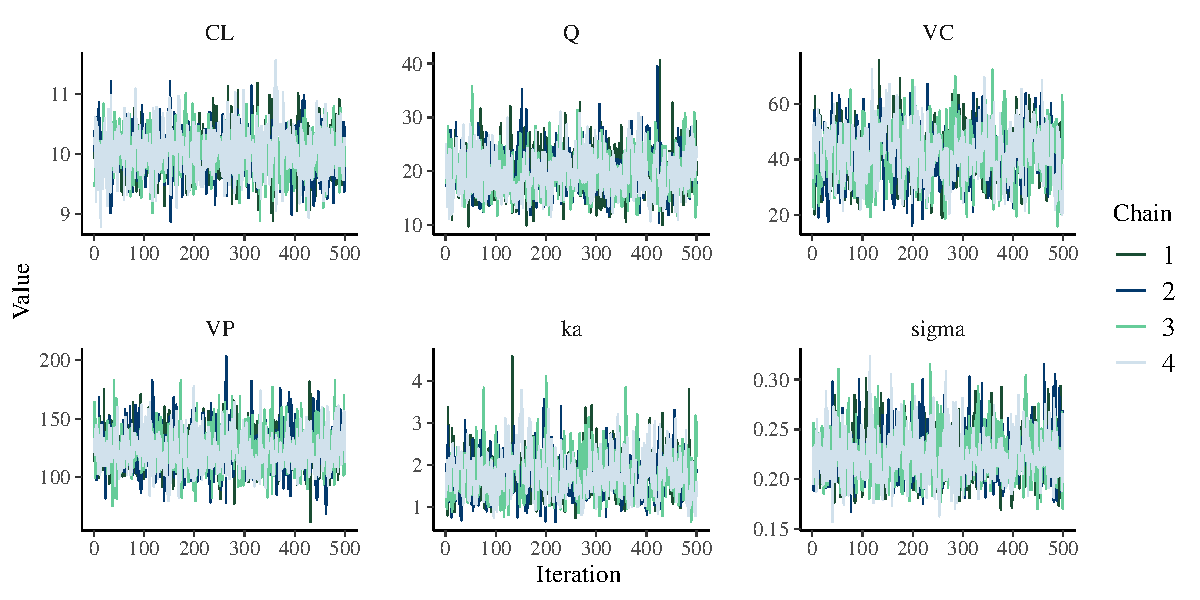
\includegraphics[width = 6in]{../figures/twocpt_traceplots_4x8.pdf}
  \caption{Trace plots. \textit{The sampled values for each parameters are plotted against the iterations during the sampling phase. Multiple Markov chains were initialized at different points. However, once in the sampling phase, we cannot distinguish them.}}
  \label{fig:trace}
  \end{center}
\end{figure}

If $\hat R \gg 1$ and, more generally, if the chains were not mixing, this would be cause for concern and an invitation to adjust our inference method.
Even when $\hat R = 1$, we should entertain the possibility that all the chains suffer from the same bias.
Stan offers additional diagnostics to identify sampling biases, notably by reporting \textit{divergent transitions} of the HMC sampler, a topic we will discuss when we fit more sophisticated models.

\subsubsection{Controlling the variance of our estimator}

Let's assume that our samples are indeed unbiased.
The expected error of our estimator is now determined by the variance.
Under certain regularity conditions, our estimator follows an MCMC central limit theorem,
\begin{equation*}
  \hat {\mathbb E} f \overset{\mathrm{approx}}{\sim} \mathrm{Normal} \left ( \mathbb E f, \frac{\mathrm{Var} f}{n_\mathrm{eff}} \right ).
\end{equation*}
where the key difference is that $\mathrm{Var} f$ is now divided by the \textit{effective sample size}, $n_\mathrm{eff}$, rather than the sample size.
This change accounts for the fact our samples are not independent: their correlation induces a loss in information, which increase the variance of our estimator.
For $CL$, we have 2,000 samples, but the effective sample size is 1,580 (Table~\ref{tab:summary}).
If $n_\mathrm{eff}$ is low, our estimator may not be precise enough and we should generate more samples.

The effective sample size is only formally defined in the context of estimators for expectation values.
We may also be interested in tail quantities, such as extreme quantiles, which are much more difficult to estimate and require many more samples to achieve a desired precision.
\citet{Vehtari:2020} propose a generalization of the effective sample size for such quantities, and introduce the \textit{tail effective sample size}.
This is to be distinguished from the traditional effective sample size, henceforth the \textit{bulk effective sample size}.
Both quantities are reported by Stan.

\subsection{Checking the model: posterior predictive checks}  \label{sec:twoCpt_ppc}

Once we develop enough confidence in our inference, we still want to check our fitted model.
There are many ways of doing this.
We may look at the posterior distribution of an interpretable parameter and see if it suggests implausible values.
Or we may evaluate the model's ability to perform a certain task, e.g. classification or prediction, as is often done in machine learning.
In practice, we find it useful to do \textit{posterior predictive
  checks} (PPC), that is simulate data from the fitted model and compare the simulation to the observed data \cite[chapter 6]{Gelman:2013}.
%
Mechanically, the procedure is straightforward:
\begin{enumerate}
  \item Draw the parameters from their posterior, $\tilde \theta \sim p(\theta \mid y).$
  \item Draw new observations from the likelihood, conditional on the drawn parameters, $\tilde y \sim p(y \mid \tilde \theta)$.
\end{enumerate}
This amounts to drawing observations from their posterior distribution, that is $\tilde y \sim p(\tilde y \mid y)$.
The uncertainty due to our estimation and the uncertainty due to our measurement error are then propagated to our predictions.

Stan provides a \texttt{generated quantities} block, which allows us to compute values, based on sampled parameters.
In our two compartment model example, the following code draws new observations from the likelihood:
\begin{lstlisting}
generated quantities {
  real concentrationObsPred[nObs] 
    = lognormal_rng(log(concentrationHat[iObs]), sigma);
}
\end{lstlisting}
%
Here, we generated predictions at the observed points for each sampled point, $\theta^{(i)}$.
This gives us a sample of predictions and we can use the $5^\mathrm{th}$ and $95^\mathrm{th}$ quantiles to construct a credible interval.
We may then plot the observations and the credible intervals (Figure~\ref{fig:ppc}) and see that, indeed, the data generated by the model is consistent with the observations.
 
\begin{figure}
  \begin{center}
  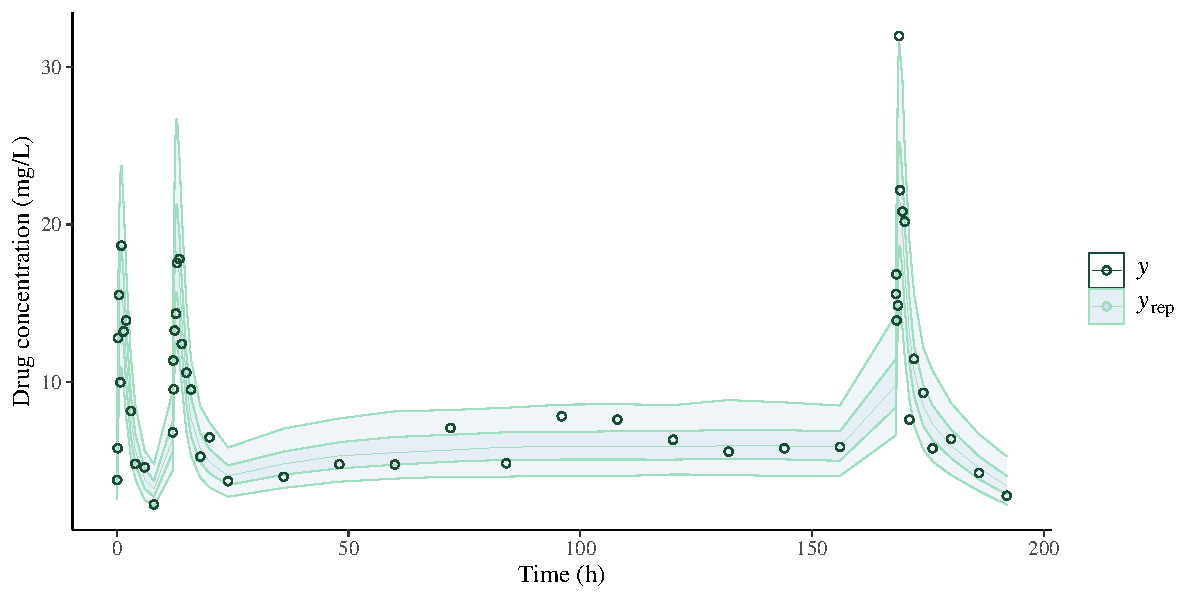
\includegraphics[width=6in]{../figures/twocpt_ppc_4x8.pdf}
  \end{center}
  \caption{Posterior predictive checks for two compartment model. \textit{The circles represent the observed data and the shaded areas the $50^\mathrm{th}$ and $90^\mathrm{th}$ credible intervals based on posterior draws.}}
  \label{fig:ppc} 
\end{figure}

\subsection{Comparing models: leave-one-out cross validation}

Beyond model criticism, we may be interested in model comparison.
Continuing our running example, we compare our two compartment model to a one compartment model, which is also supported by Torsten via the \texttt{pmx\_solve\_onecpt} routine.
The corresponding posterior predictive checks are shown in Figure~\ref{fig:ppc_onecpt}.

\begin{figure}
  \begin{center}
  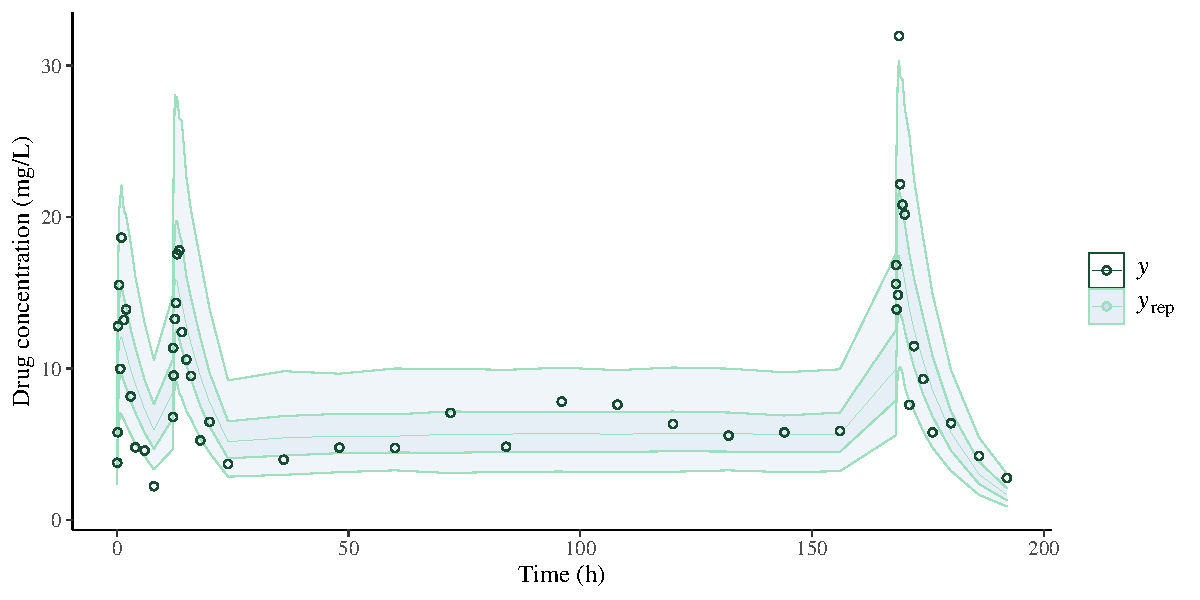
\includegraphics[width=6in]{../figures/onecpt_ppc_4x8.pdf}
  \end{center}
  \caption{Posterior predictive checks for one compartment model. \textit{The circles represent the observed data and the shaded areas the $50^\mathrm{th}$ and $90^\mathrm{th}$ credible intervals based on posterior draws. A graphical inspection suggests the credible interval is wider for the one compartment model than they are for the two compartment model.}}
  \label{fig:ppc_onecpt} 
\end{figure}

There are several ways of comparing models and which method is appropriate crucially depends on the insights we wish to gain.
If our goal is to asses a model's ability to make good out-of-sample predictions, we may consider \textit{Bayesian leave-one-out} (LOO) cross validation.
The premise of cross-validation is to exclude a point, $(y_i, x_i)$, from the \textit{training set}, i.e. the set of data to which we fit the model.
Here $x_i$ denotes the covariate and in our example, the relevant row in the event schedule.
We denote the reduced data set, $y_{-i}$.
We then generate a prediction $(\tilde y_i, x_i)$ using the fitted model, and compare $\tilde y_i$ to $y_i$.
A classic metric to make this comparison is the squared error, $(\tilde y_i - y_i)^2$.

Another approach is to use the \textit{LOO estimate of out-of-sample predictive fit}:
\begin{equation*}
  \mathrm{elp}_\mathrm{loo} := \sum_{i}^n \log p(y_i \mid y_{-i}).
\end{equation*}
%
Here, no prediction is made.
We however examine how consistent an ``unobserved'' data point is with our fitted model.
Computing this estimator is expensive, since it requires fitting the model to $n$ different training sets in order to evaluate each term in the sum.

\citet{Vehtari:2016} propose an estimator of $\mathrm{elp}_\mathrm{loo}$, which uses Pareto smooth importance sampling and only requires a single model fit.
The premise is to compute
\begin{equation*}
  \log p(y_i \mid y)
\end{equation*}
and correct this value, using importance sampling, to estimate $\log p(y_i \mid y_{-i})$.
Naturally this estimator may be inaccurate.
What makes this tool so useful is that we can use the Pareto shape parameter, $\hat k$, to asses how reliable the estimate is.
In particular, if $\hat k > 0.7$, then the estimate shouldn't be trusted.
The estimator is implemented in the R package Loo \cite{Gabry:2020}.

Conveniently, we can compute $\log p(y_i \mid y)$ in Stan's \texttt{generated quantities} block.
\begin{lstlisting}
vector[nObs] log_lik;
for (i in 1:nObs)
  log_lik[i] = 
   lognormal_lpdf(cObs[i] | log(concentrationHat[iObs]),
                  sigma);
\end{lstlisting}
These results can then be extracted and fed into Loo to compute $\mathrm{elp}_\mathrm{loo}$.
The file \texttt{twoCpt.r} in the Supplementary Material shows exactly how to do this.
Figure~\ref{fig:loo} plots the estimated $\mathrm{elp}_\mathrm{loo}$, along with a standard deviation, and shows the two compartment model has better out-of-sample predictive capabilities.

\begin{figure}
  \begin{center}
    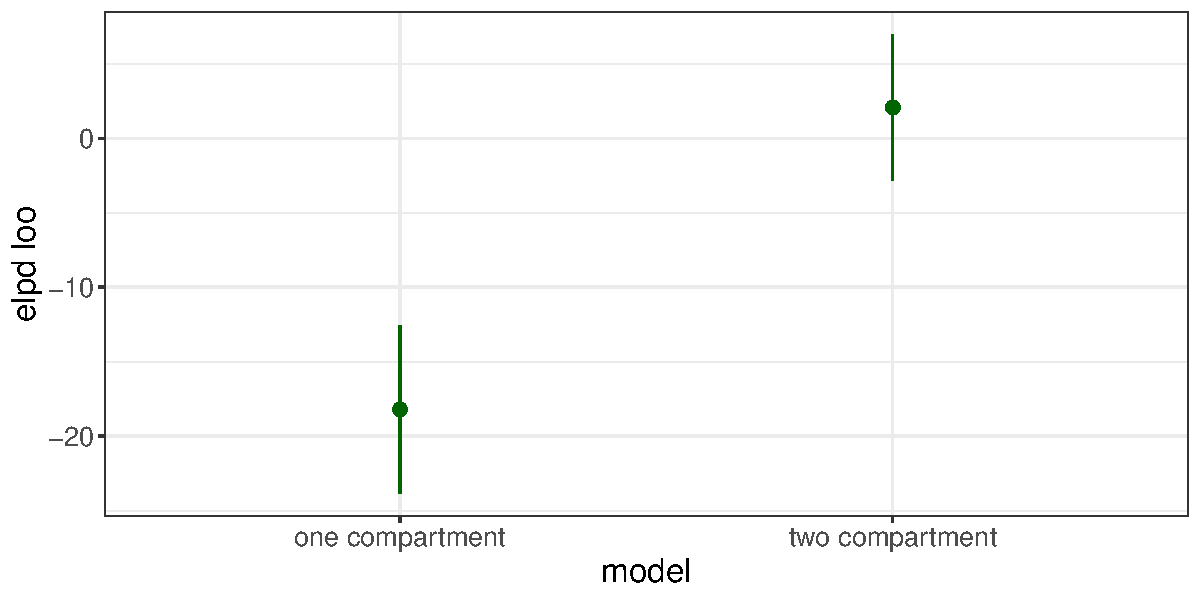
\includegraphics[width = 5in]{../figures/elpd_loo_comp_4x8.pdf}
    \caption{Leave-one-out estimate of out-of-sample predictive fit. \textit{Plotted is the estimate, $\mathrm{elp}_\mathrm{loo}$, for the one and two compartment models. Clearly, the two compartment models has superior predictive capabilities.}}
    \label{fig:loo}
  \end{center}
\end{figure}


